% ─────────────────────────────────────────────────────────────────────────────
% FRISBEE — Project Report
% Engine : pdfLaTeX
% Font   : newtxtext + newtxmath on Overleaf
%          mathpazo used here for local compilation only
% ─────────────────────────────────────────────────────────────────────────────
\documentclass[11pt, a4paper]{report}

% ── Encoding ─────────────────────────────────────────────────────────────────
\usepackage[T1]{fontenc}
\usepackage[utf8]{inputenc}

% ── Font (swap for Overleaf: replace these two lines with newtxtext,newtxmath)
\usepackage{mathpazo}
\linespread{1.05}

% ── Microtypography ──────────────────────────────────────────────────────────
\usepackage[protrusion=true, expansion=false]{microtype}

% ── Page geometry ────────────────────────────────────────────────────────────
\usepackage[
  top    = 1.10in,
  bottom = 1.10in,
  left   = 1.25in,
  right  = 1.00in
]{geometry}

% ── Mathematics ──────────────────────────────────────────────────────────────
\usepackage{amsmath, amssymb}

% ── Colour — CMYK throughout ─────────────────────────────────────────────────
\usepackage[cmyk]{xcolor}
\definecolor{accent}   {cmyk}{0.58, 0.00, 0.18, 0.57}   % #2E6E5A
\definecolor{accentbg} {cmyk}{0.03, 0.00, 0.01, 0.03}   % #F0F7F4
\definecolor{ltborder} {cmyk}{0.07, 0.00, 0.02, 0.15}   % #C8D8D4
\definecolor{textmid}  {cmyk}{0.00, 0.00, 0.00, 0.55}
\definecolor{textlight}{cmyk}{0.00, 0.00, 0.00, 0.38}

% ── TikZ ─────────────────────────────────────────────────────────────────────
\usepackage{tikz}
\usetikzlibrary{positioning, calc, fit, backgrounds,
                shapes.geometric, arrows.meta}
\pgfdeclarelayer{background}
\pgfsetlayers{background,main}

\tikzset{
  modbox/.style={
    rectangle, rounded corners=2.5pt,
    draw=ltborder, fill=white,
    minimum width=4.9cm, minimum height=0.78cm,
    align=center, inner sep=5pt, font=\small
  },
  smallbox/.style={
    rectangle, rounded corners=2.5pt,
    draw=ltborder, fill=white,
    minimum width=2.1cm, minimum height=0.78cm,
    align=center, inner sep=4pt, font=\footnotesize
  },
  primbox/.style={
    rectangle, rounded corners=2.5pt,
    draw=accent, fill=accentbg,
    minimum width=4.9cm, minimum height=0.78cm,
    align=center, inner sep=5pt, font=\small
  },
  busbox/.style={
    rectangle, rounded corners=3pt, fill=accent,
    minimum width=5.4cm, minimum height=0.90cm,
    align=center, font=\small
  },
  decision/.style={
    diamond, aspect=2.6, draw=black!70, fill=white,
    minimum width=3.0cm, align=center, font=\small
  },
  arr/.style  = {-Stealth, thick, color=accent},
  darr/.style = {-Stealth, dashed, thin, color=black!28},
}

% ── Tables ───────────────────────────────────────────────────────────────────
\usepackage{booktabs, tabularx, array}
\renewcommand{\arraystretch}{1.16}

% ── Figures ──────────────────────────────────────────────────────────────────
\usepackage{graphicx, float}
\usepackage{caption}
\captionsetup{font=small, labelfont=bf, labelsep=period, skip=6pt}

% ── Section styling ──────────────────────────────────────────────────────────
\usepackage{titlesec}

\titleformat{\chapter}[hang]
  {\normalfont\Large\bfseries}
  {\thechapter.}{0.5em}{}
  [\vspace{3pt}{\color{accent}\rule{\textwidth}{0.45pt}}\vspace{-2pt}]
\titlespacing*{\chapter}{0pt}{0pt}{16pt}

\titleformat{\section}
  {\normalfont\large\bfseries}{\thesection}{0.7em}{}
\titlespacing{\section}{0pt}{14pt}{4pt}

\titleformat{\subsection}
  {\normalfont\normalsize\bfseries}{\thesubsection}{0.6em}{}
\titlespacing{\subsection}{0pt}{10pt}{3pt}

% ── Headers / footers ────────────────────────────────────────────────────────
\usepackage{fancyhdr}
\pagestyle{fancy}
\fancyhf{}
\fancyhead[L]{\small\itshape FRISBEE}
\fancyhead[R]{\small\itshape Dept.\ of AI \& ML, NHCE}
\fancyfoot[C]{\small\thepage}
\renewcommand{\headrulewidth}{0.35pt}
\renewcommand{\footrulewidth}{0pt}

% ── Lists ────────────────────────────────────────────────────────────────────
\usepackage{enumitem}
\setlist{noitemsep, topsep=3pt, leftmargin=*}

% ── Paragraph rhythm ─────────────────────────────────────────────────────────
\setlength{\parindent}{0pt}
\setlength{\parskip}{5pt}

% ── Algorithm ────────────────────────────────────────────────────────────────
\usepackage{algorithm, algpseudocode}

% ── Citations — Harvard author-year ──────────────────────────────────────────
\usepackage[round, authoryear, sort]{natbib}

% ── Hyperref ─────────────────────────────────────────────────────────────────
\usepackage{hyperref}
\hypersetup{pdfborder={0 0 0},
            pdftitle={FRISBEE}, pdfauthor={Bhavishya Srivastava et al.}}

% ─────────────────────────────────────────────────────────────────────────────
\begin{document}
\pagestyle{plain}

% ── COVER PAGE ───────────────────────────────────────────────────────────────
\begin{titlepage}
\centering
\vspace*{0.8cm}


\includegraphics[height=2.5cm]{nhce_logo.png}

\vspace{0.55cm}
{\fontsize{13.5}{17}\selectfont\bfseries NHCE, Bangalore, KA, India}\\[3pt]
{\small Department of Artificial Intelligence \& Machine Learning}\\[2pt]


\vspace{0.5cm}
{\color{accent}\rule{0.52\textwidth}{0.45pt}}
\vspace{1.1cm}

{\fontsize{32}{38}\selectfont\bfseries FRISBEE}\\[10pt]
{\fontsize{12}{16}\selectfont\itshape
  Functional Realtime Intelligence for Spotting\\[2pt]
  Blissful Everyday Actions}

\vspace{0.5cm}
{\color{accent}\rule{0.52\textwidth}{0.45pt}}
\vspace{0.9cm}

{\small\color{textmid}\itshape
  A personal logistic regression model trained on daily free-form text\\[2pt]
  to predict individual weekly behavioural alignment.}

\vspace{1.6cm}

{\small
\begin{tabular}{@{}ll@{}}
  Bhavishya Srivastava & 1NH24AI197 \\[4pt]
  Arya Navaneeth       & 1NH24AI217 \\[4pt]
  AJL Hansika          & 1NH24AI216 \\[4pt]
  Vunnam Manogna       & 1NH24AI211 \\
\end{tabular}}

\vspace{1.3cm}

{\small
  Guide: Senior Assistant Prof.\ Shashikala K S\\[4pt]
  Mini Project -- I (24AIM48)\quad\textperiodcentered\quad 2025--26}

\vfill
{\scriptsize\color{textmid}
  \href{https://myfrisbee.lovable.app}{myfrisbee.lovable.app}
}

\end{titlepage}

% ── CERTIFICATE ──────────────────────────────────────────────────────────────
\newpage\thispagestyle{plain}
\vspace*{1.4cm}
\begin{center}

  {\Large\bfseries Certificate}\\[7pt]
  {\color{accent}\rule{0.38\textwidth}{0.4pt}}
\end{center}
\vspace{0.9cm}

This is to certify that the project \textbf{FRISBEE: Functional Realtime
Intelligence for Spotting Blissful Everyday Actions} was carried out by
Bhavishya Srivastava (1NH24AI197), Arya Navaneeth (1NH24AI217), AJL Hansika
(1NH24AI216), and Vunnam Manogna (1NH24AI211) as part of Mini Project -- I
(24AIM48) in the Department of Artificial Intelligence and Machine Learning,
New Horizon College of Engineering, Bangalore, during the academic year
2025--26. The work is original and was completed under the guidance of the
undersigned.

\vspace{3.2cm}

\begin{tabular}{@{}p{6.2cm}p{6.2cm}@{}}
  \rule{5.4cm}{0.3pt}            & \rule{5.4cm}{0.3pt}           \\[5pt]
  \textbf{Prof.\ Shashikala K S} & \textbf{Dr.\ N V Uma Reddy}   \\
  Project Guide                  & Head of Department             \\
  Dept.\ of AI \& ML, NHCE      & Dept.\ of AI \& ML, NHCE      \\
\end{tabular}

\vspace{2.2cm}

\begin{tabular}{@{}p{6.2cm}@{}}
  \rule{5.4cm}{0.3pt} \\[5pt]
  \textbf{External Examiner}
\end{tabular}

% ── ACKNOWLEDGEMENT ──────────────────────────────────────────────────────────
\newpage\thispagestyle{plain}
\vspace*{1.4cm}
\begin{center}
  {\Large\bfseries Acknowledgement}\\[7pt]
  {\color{accent}\rule{0.38\textwidth}{0.4pt}}
\end{center}
\vspace{0.9cm}

We thank \textbf{Prof.\ Shashikala K S} for guiding this project. Her
questions consistently pushed us toward greater precision, and her
patience gave us room to build something we genuinely care about.

We thank \textbf{Dr.\ N V Uma Reddy} and the Department of Artificial
Intelligence and Machine Learning for an environment that takes
project-based learning seriously.

The technical foundation of this work rests on Karen Sparck Jones's 1972
paper on inverse document frequency, still one of the most elegant results
in information retrieval. We also draw on research by Daniel Kahneman,
Tali Sharot, and David Dunning, whose work on prediction, optimism bias,
and self-assessment defined the problem we set out to address.

\vspace{1.8cm}
\begin{flushright}
  Bhavishya Srivastava\\
  Arya Navaneeth\\
  AJL Hansika\\
  Vunnam Manogna\\[5pt]
  \textit{Summer, 2026}
\end{flushright}

% ── ABSTRACT ─────────────────────────────────────────────────────────────────
\newpage\thispagestyle{plain}
\vspace*{1.4cm}
\begin{center}
  {\Large\bfseries Abstract}\\[7pt]
  {\color{accent}\rule{0.38\textwidth}{0.4pt}}
\end{center}
\vspace{0.9cm}

People routinely overestimate how well they will behave in the coming
week. This is not random error. It is a consistent, measurable bias
rooted in how humans construct self-predictions: drawing on idealised
self-concept rather than behavioural history. No existing tool attempts
to learn this gap from a single person's own words.

FRISBEE is a browser-based system in which a logistic regression model,
trained exclusively on one user's daily free-form messages, predicts
whether each week will be one of behavioural alignment or not. Each
message is converted into a four-dimensional feature vector via
cluster-weighted TF-IDF scoring across four semantic dimensions:
\textit{drift}, \textit{align}, \textit{excuse}, and \textit{energy}.
A blended inverse document frequency formula, combining personal and
background corpus statistics, resolves the cold-start problem in the
early weeks of use. At the end of each week, the model's prediction is
compared against the user's own blinded self-prediction in a direct
duel. Over time the model learns the user's specific language patterns,
and by extension, their specific optimism bias.

All computation runs on the user's device. No data is transmitted.
The system is implemented as a zero-dependency TypeScript ML pipeline
and deployed as a live web application.

\vspace{0.6cm}
\noindent\textbf{Keywords:}\enspace
logistic regression,\enspace TF-IDF,\enspace behavioural prediction,\enspace
optimism bias,\enspace on-device machine learning

% ── FRONT MATTER ─────────────────────────────────────────────────────────────
\newpage
\tableofcontents

\newpage
\listoffigures

\newpage
\listoftables

\newpage
\pagestyle{fancy}
\setcounter{page}{1}

% ─────────────────────────────────────────────────────────────────────────────
\chapter{Introduction}
% ─────────────────────────────────────────────────────────────────────────────

\section{Background}

There is a consistent gap between how people predict their own behaviour and
how they actually behave. Research in cognitive psychology and decision science
has established that self-predictions draw on idealised self-concept rather
than behavioural history, producing estimates that are systematically biased.
\citet{sharot2011} identified this as the optimism bias: a universal tendency
to overestimate the probability of positive future outcomes. \citet{dunning2004}
demonstrated that the failure is not simply a lack of information. Even when
people have direct access to their own past behaviour, they do not consult it
when forming predictions about themselves. The estimate is constructed from
how a person thinks about themselves, not from evidence of how they have acted.

This pattern is most visible in adolescents. The teenage years involve rapid
change in identity and self-concept, and the distance between aspiration and
action is felt acutely. The everyday language of this experience is precise:
\textit{I said I would study and did not.} \textit{Why do I keep doing this.}
These are not productivity complaints. They are observations about a gap
between who a person imagines themselves to be and who actually shows up.
FRISBEE takes this gap seriously as a research problem and asks whether it
is learnable from the person's own words.

\section{Problem Statement}

Self-prediction of weekly behaviour fails in a specific and exploitable way.
The prediction is formed from self-concept, not from evidence. The language a
person uses each day, however, is closer to evidence. Words like
\textit{procrastinated}, \textit{exhausted}, \textit{finally finished}, and
\textit{pumped} are not arbitrary choices. They reflect the actual state of
the day as the person experienced it, written close to the time of the
experience.

The central question this project addresses is: given a person's daily
free-form messages over several weeks, can a machine learning model trained
exclusively on those messages predict whether any given week was one of
behavioural alignment more accurately than the person can predict it
themselves?

\section{Objectives}

\begin{enumerate}
  \item Design a text feature extraction pipeline that converts free-form daily
    messages into a four-dimensional feature vector via cluster-weighted
    TF-IDF with a blended inverse document frequency formula.

  \item Build a logistic regression model with L2 regularisation that trains
    incrementally on one user's labelled weekly data, with no external
    training corpus and no pre-trained weights.

  \item Implement a weekly prediction duel in which the model's prediction is
    compared against the user's own blinded self-prediction, with outcome
    scores tracked over time.

  \item Implement a hypothesis surfacing module that identifies words
    statistically associated with the user's good or bad weeks using
    Bernoulli confidence estimation.

  \item Store all data locally on the user's device using IndexedDB, with no
    server component and no data transmission.

  \item Deploy the system as a functional minimum viable product and
    demonstrate the viability of individual-level behavioural alignment
    prediction from natural language.
\end{enumerate}

\section{Literature Survey}

\subsection{\citet{sweller1988} --- Cognitive Load Theory}

Sweller established that when a person's working memory is occupied, the
quality of secondary cognitive tasks degrades significantly. This finding
motivates FRISBEE's choice of free-form text input over structured tracking
forms. Dashboards and checklists impose a cognitive load through their
structure. A single open-ended daily message imposes almost none. The system
extracts structure from unstructured input rather than demanding structure
from the user.

\subsection{\citet{kahneman2011} --- Thinking, Fast and Slow}

Kahneman describes two modes of cognition. System 1 is fast, automatic,
and operates without deliberate effort. System 2 is slow and effortful.
Self-prediction tends to rely on System 1: a person generates a weekly
prediction based on how they feel about themselves in that moment. The
logistic regression model in FRISBEE functions as an external System 2
proxy. It reviews the actual words written over the week and produces a
prediction based on observed patterns, not on current mood.

\subsection{\citet{rebetez2015} --- Procrastination and Self-Regulation}

Rebetez et al.\ identify three correlated factors in procrastination
behaviour: cognitive (poor planning), emotional (difficulty regulating
negative affect), and motivational (low outcome expectancy). These factors
manifest in language. Words such as \textit{supposed to}, \textit{tired},
and \textit{tomorrow} are markers of emotional avoidance and motivational
failure. The \textit{excuse} cluster in FRISBEE's vocabulary was designed
to capture exactly this class of signal.

\subsection{\citet{anderson2003} --- Decision Avoidance}

Anderson provides a taxonomy of decision avoidance behaviours including
deferral and omission. Adolescents show elevated rates of decision avoidance
when outcomes are uncertain or when they anticipate negative emotional
consequences. FRISBEE's weekly commit mechanism addresses this by creating
a single, low-friction binary decision point at the end of each week: was
this a yes-week or a no-week?

\subsection{\citet{lee2004} --- Trust in Automation}

Lee and See identify two failure modes in human interaction with automated
systems. Over-reliance occurs when users follow automation regardless of
accuracy. Under-reliance occurs when users dismiss useful automated output.
Both degrade outcomes. The prediction duel in FRISBEE is designed to
address this: the user makes their own prediction before seeing the model's,
preventing anchoring, and the duel score over time provides calibration
evidence without requiring the user to interpret model internals.

\subsection{\citet{hengstler2016} --- Applied AI and Trust}

Hengstler et al.\ argue that trust in applied AI systems must be earned
through demonstrated reliability, not claimed upfront. FRISBEE is designed
with this in mind. The model is initialised with zero weights and makes
near-random predictions in its first few weeks. The duel score makes this
visible, allowing trust to be calibrated to actual performance.

\subsection{\citet{sparckjones1972} --- Inverse Document Frequency}

Sparck Jones introduced inverse document frequency as a measure of term
specificity. A term appearing in many documents provides less information
than one appearing in few. This is the foundation of the IDF component in
FRISBEE's feature extractor. Words a user writes every day carry no
alignment signal. A word they rarely use, but wrote today, carries
significant information about what kind of day it was.

\subsection{\citet{salton1988} --- Term-Weighting in Retrieval}

Salton and Buckley evaluated term-weighting schemes systematically,
establishing TF-IDF as a computationally efficient and reliable method for
encoding document content. Their analysis confirms that combining local
term frequency with global term specificity produces more informative
representations than either component alone, which FRISBEE applies directly.

\subsection{\citet{sharot2011} --- The Optimism Bias}

Sharot established the optimism bias as one of the most consistent findings
in cognitive science: people across cultures systematically overestimate
positive future outcomes. The bias is structural, tied to how the brain
constructs self-predictions. FRISBEE operationalises this finding. The gap
between a user's self-prediction and the model's prediction is, in aggregate,
a measure of their personal optimism bias magnitude.

\subsection{\citet{dunning2004} --- Flawed Self-Assessment}

Dunning, Heath, and Suls review evidence that people are systematically poor
judges of their own behaviour, even with access to their own history.
Self-assessments are constructed rather than retrieved: people generate an
estimate from self-concept rather than consulting their record. FRISBEE
bypasses this construction process. The model is trained on the actual
behavioural record, not on the user's narrative about it.

\section{Existing Systems}

Table~\ref{tab:existing} surveys the tools most relevant to FRISBEE's
problem space and identifies where each falls short.

\begin{table}[H]
\centering
\caption{Comparison of existing approaches}
\label{tab:existing}
\begin{tabularx}{\textwidth}{@{} p{3.0cm} p{3.4cm} X @{}}
\toprule
\textbf{System type} & \textbf{Approach} & \textbf{Limitation} \\
\midrule
Habit trackers
  & Binary daily completion counts
  & No language analysis, no prediction, no model of the
    intention-to-action gap. \\[6pt]
Journaling apps
  & Free-form text storage for recall
  & No modelling. Any ``insight'' relies on population-trained
    sentiment classifiers applied to the individual. \\[6pt]
Sentiment APIs
  & Pre-trained affect classification
  & Models trained on crowd data. Individual patterns are averaged
    away. Not predictive of future outcomes. \\[6pt]
Goal dashboards
  & Structured progress tracking
  & Require structured input. Do not learn from language and do
    not predict future alignment. \\
\bottomrule
\end{tabularx}
\end{table}

The common failure is that all existing approaches are either built for
populations or require structured input. None learns from a single user's
unstructured language, and none models the intention-to-action gap at the
individual level.

\section{Proposed System}

FRISBEE is a browser-based application in which a logistic regression model
is trained exclusively on one user's daily free-form messages. The model
converts each message into a feature vector using four hand-designed semantic
clusters and blended TF-IDF scoring, then predicts weekly behavioural
alignment as a binary outcome. At the end of each week the user commits a
self-prediction, the model reveals its own, and the user provides the ground
truth label. The model then trains on the week's messages and updates its
weights accordingly.

All computation and storage occur on the user's device. No data is
transmitted. The system becomes more accurate as the user's personal corpus
accumulates, learning the specific words and patterns that predict alignment
for that person and no one else.

% ─────────────────────────────────────────────────────────────────────────────
\chapter{System Requirements}
% ─────────────────────────────────────────────────────────────────────────────

\section{Hardware Requirements}

FRISBEE is a client-side web application. There are no server-side hardware
requirements. Table~\ref{tab:hardware} lists the requirements for the device
running the application.

\begin{table}[H]
\centering
\caption{Hardware requirements}
\label{tab:hardware}
\begin{tabularx}{\textwidth}{@{} p{2.8cm} X @{}}
\toprule
\textbf{Component} & \textbf{Requirement} \\
\midrule
Processor
  & Any processor capable of running a modern web browser.
    No specific instruction set is required. \\[5pt]
Memory
  & Minimum 2\,GB RAM. 4\,GB is recommended for comfortable
    browser performance alongside other applications. \\[5pt]
Storage
  & Minimum 50\,MB available for IndexedDB. Typical usage over
    one year of daily messages is under 5\,MB. \\[5pt]
Display
  & Any screen capable of rendering a modern browser.
    The application targets a mobile-first viewport of
    approximately 390\,px width. \\[5pt]
Network
  & An internet connection is required only for the initial
    application load. All subsequent computation and storage
    are fully offline. \\
\bottomrule
\end{tabularx}
\end{table}

\section{Software Requirements}

Table~\ref{tab:software} lists the software components required for
development and deployment.

\begin{table}[H]
\centering
\caption{Software requirements}
\label{tab:software}
\begin{tabularx}{\textwidth}{@{} p{2.8cm} X @{}}
\toprule
\textbf{Component} & \textbf{Requirement} \\
\midrule
Web browser
  & Any browser supporting IndexedDB, the Web Audio API, and
    ES2022 JavaScript. Tested on Chrome 120+, Firefox 121+,
    and Safari 17+. \\[5pt]
Dev runtime
  & Bun 1.x or Node.js 20+ for local development and build.
    Not required by end users. \\[5pt]
Build tool
  & Vite 7, included in project dependencies. \\[5pt]
Language
  & TypeScript 5.8, compiled to ES modules. No TypeScript
    runtime dependency in production. \\[5pt]
Deployment
  & Any static file host or edge worker runtime. No
    server-side runtime required. \\
\bottomrule
\end{tabularx}
\end{table}

\section{Key Dependencies}

The application uses no external machine learning library. The complete ML
pipeline is implemented in plain TypeScript. The following third-party
libraries handle non-ML responsibilities.

\begin{itemize}
  \item \textbf{idb} --- Promise-based IndexedDB wrapper. Used exclusively
    in \texttt{vault.ts} for data persistence.
  \item \textbf{Zustand} --- Lightweight React state management. Used in
    \texttt{brain.ts} for the mascot state machine.
  \item \textbf{TanStack Router} --- File-based routing for the five
    application routes.
  \item \textbf{React 19} --- UI rendering. No React-specific data
    processing.
  \item \textbf{Tailwind CSS v4} --- Utility-class styling with no
    effect on application logic.
\end{itemize}

% ─────────────────────────────────────────────────────────────────────────────
\chapter{System Design}
% ─────────────────────────────────────────────────────────────────────────────

\section{Architecture}

The system is split into two independent modules that share no direct
imports, as shown in Figure~\ref{fig:arch}. The prediction pipeline (\texttt{src/lib/frisbee/}) handles all
machine learning and data management. The UX layer (\texttt{src/lib/buddy/})
handles feedback to the user: mascot behaviour, sound, and haptics. The two
modules communicate only through a typed event bus. This separation means
the ML pipeline can be reasoned about and tested entirely independently of
the interface layer.

\begin{figure}[H]
\centering
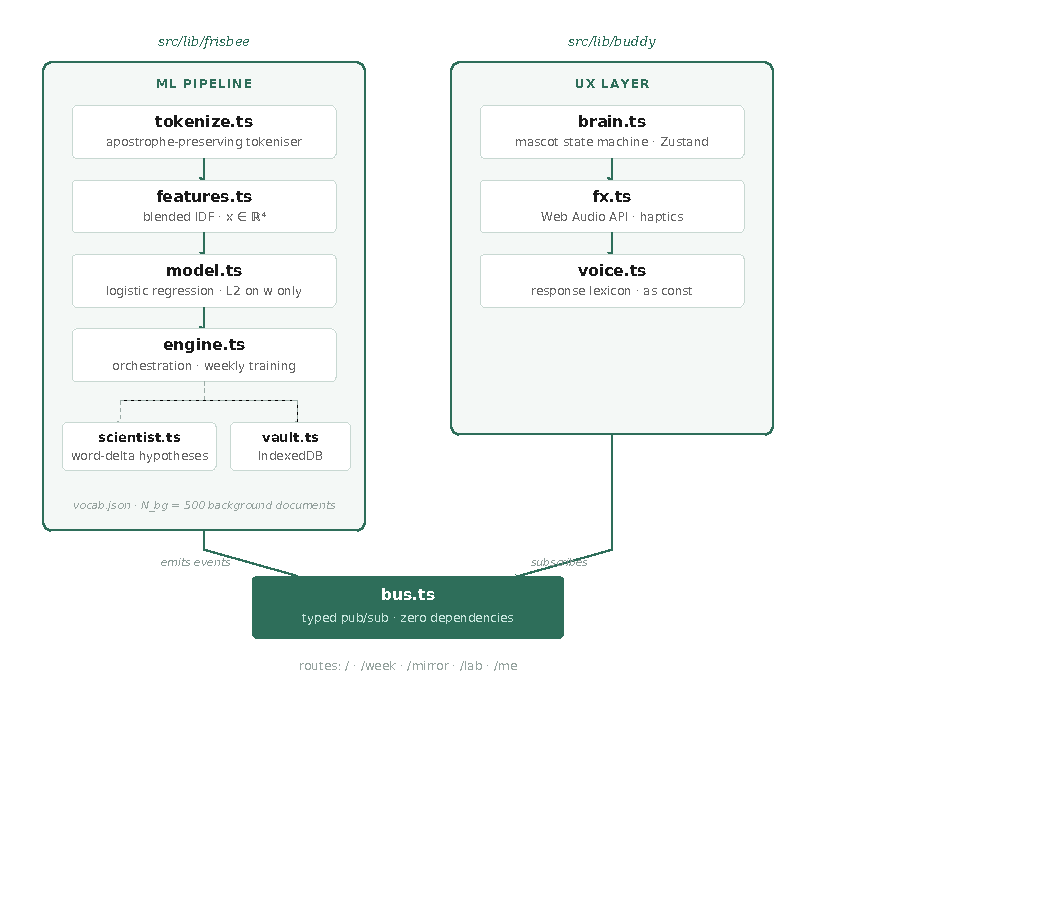
\includegraphics[width=0.92\textwidth, trim=0 104 0 0, clip]{fig_architecture}
\caption{System architecture. The two modules communicate only through the typed event bus.}
\label{fig:arch}
\end{figure}

\section{Tokenisation}

The tokeniser in \texttt{tokenize.ts} converts raw text to a list of
lowercase tokens while preserving apostrophes inside words. The design
criterion is the preservation of contractions. The word \textit{didn't}
belongs to the \textit{excuse} cluster. A naive tokeniser that strips
punctuation splits it into \textit{didn} and \textit{t}, both of which
match nothing. The signal is lost.

The tokeniser applies three transformations in order. First, the input is
lowercased. Second, Unicode apostrophe variants (\textsc{u+2018},
\textsc{u+2019}, \textsc{u+02bc}) are replaced with the standard ASCII
apostrophe, handling mobile keyboard input. Third, the regular expression

\begin{equation}
  \texttt{/[a-z0-9][a-z0-9']*[a-z0-9]\,|\,[a-z0-9]/g}
\end{equation}

extracts tokens. This pattern permits apostrophes only in the interior of a
token, not at its boundaries, so contractions are preserved while
surrounding punctuation is discarded correctly.

\section{Feature Extraction}

\subsection{Cluster Vocabulary}

The vocabulary in \texttt{vocab.json} defines four semantic clusters.
Table~\ref{tab:clusters} lists representative words from each.

\begin{table}[H]
\centering
\caption{Semantic clusters with representative words}
\label{tab:clusters}
\begin{tabularx}{\textwidth}{@{} p{1.8cm} X @{}}
\toprule
\textbf{Cluster} & \textbf{Words (sample)} \\
\midrule
drift
  & procrastinated, scrolled, wasted, avoided, snoozed, skipped,
    forgot, didn't, nothing, again \\[4pt]
align
  & focused, finished, shipped, studied, built, completed, proud,
    actually, finally, crushed \\[4pt]
excuse
  & tired, exhausted, tomorrow, later, busy, overwhelmed, but,
    almost, should, couldn't \\[4pt]
energy
  & motivated, pumped, inspired, excited, happy, great, lit,
    grateful, let's, locked \\
\bottomrule
\end{tabularx}
\end{table}

Words may belong to more than one cluster. The words \textit{couldn't},
\textit{didn't}, and \textit{wouldn't} appear in both \textit{drift} and
\textit{excuse}. The words \textit{locked} and \textit{crushing} appear in
both \textit{align} and \textit{energy}. Such words contribute their
TF-IDF score to every cluster they belong to.

\subsection{TF-IDF Computation}

For each token $w$ in a submitted message, the term frequency is:
\begin{equation}
  \mathrm{TF}(w) = \frac{\mathrm{count}(w)}{\text{total tokens}}
\end{equation}

The personal IDF, given the user's accumulated corpus of $N_p$ messages
with document frequency $df_p(w)$, is:
\begin{equation}
  \mathrm{IDF}_p(w) = \log\!\left(\frac{N_p + 1}{df_p(w) + 1}\right) + 1
\end{equation}

The background IDF is pre-computed over a corpus of $N_{bg} = 500$
documents stored in \texttt{vocab.json}. For words absent from the
background corpus, $df_{bg}(w) = 1$ (not zero):
\begin{equation}
  \mathrm{IDF}_{bg}(w) = \log\!\left(\frac{N_{bg} + 1}{df_{bg}(w) + 1}
  \right) + 1
\end{equation}

The blended IDF is a weighted average, with weights proportional to the
respective corpus sizes:
\begin{equation}
  \mathrm{IDF}_{blend}(w)
  = \frac{N_p \cdot \mathrm{IDF}_p(w) + N_{bg} \cdot \mathrm{IDF}_{bg}(w)}
         {N_p + N_{bg}}
  \label{eq:blend}
\end{equation}

When $N_p = 0$ (no messages yet), equation~\eqref{eq:blend} reduces to
$\mathrm{IDF}_{bg}(w)$, providing non-zero feature values from day one.
As $N_p$ grows, the personal IDF progressively dominates the blend. This
resolves the cold-start problem without requiring any minimum usage period.

The score for cluster $c$ is the sum of TF-IDF weights over all tokens in
the message that belong to that cluster:
\begin{equation}
  x_c = \sum_{w \,\in\, \text{msg} \,\cap\, C_c}
        \mathrm{TF}(w) \cdot \mathrm{IDF}_{blend}(w)
\end{equation}

The full feature vector is:
\begin{equation}
  \mathbf{x}
  = \bigl[x_{\mathrm{drift}},\;
    x_{\mathrm{align}},\;
    x_{\mathrm{excuse}},\;
    x_{\mathrm{energy}}\bigr]
  \in \mathbb{R}^4
\end{equation}

\section{The Logistic Regression Model}

\subsection{Forward Pass}

The model maintains a weight vector $\mathbf{w} \in \mathbb{R}^4$ and
a scalar bias $b \in \mathbb{R}$, both initialised to zero. The linear
combination is:
\begin{equation}
  z = \mathbf{w}^\top \mathbf{x} + b
    = \sum_{i=1}^{4} w_i\, x_i + b
\end{equation}

The value $z$ is clipped to $[-500,\, 500]$ before the sigmoid to prevent
floating-point overflow. The prediction is:
\begin{equation}
  \hat{p} = \sigma(z) = \frac{1}{1 + e^{-z}}, \qquad \hat{p} \in (0,1)
\end{equation}

A binary prediction is obtained by thresholding at 0.5. The value
$\hat{p}$ is the model's estimate of the probability that the current
week is a yes-week.

\subsection{Loss and Parameter Update}

After the user provides the ground truth label $y \in \{0, 1\}$ at the
end of the week, the loss is binary cross-entropy:
\begin{equation}
  \mathcal{L}
  = -\bigl[y \log\hat{p} + (1-y)\log(1-\hat{p})\bigr]
\end{equation}

The gradient of $\mathcal{L}$ with respect to $\mathbf{w}$ is:
\begin{equation}
  \frac{\partial \mathcal{L}}{\partial \mathbf{w}}
  = (\hat{p} - y)\,\mathbf{x}
\end{equation}

This is the defining result of logistic regression: the gradient is the
prediction error times the input. With L2 regularisation on the weights,
the update rule for each weight is:
\begin{equation}
  w_i \;\leftarrow\; w_i
  - \eta\bigl[(\hat{p} - y)\,x_i + \lambda\, w_i\bigr],
  \quad i = 1,2,3,4
\end{equation}

The bias is updated without regularisation:
\begin{equation}
  b \;\leftarrow\; b - \eta\,(\hat{p} - y)
\end{equation}

The hyperparameters are fixed at $\eta = 0.1$ (learning rate) and
$\lambda = 0.01$ (L2 strength). The bias is excluded from regularisation
deliberately. Penalising $b$ would pull predictions toward $\hat{p} = 0.5$
regardless of the evidence. The bias encodes the user's personal base
rate of yes-weeks, which is genuine signal and must not be suppressed.

The engine applies one gradient step per daily message in the week,
running them in chronological order. If the user submitted messages on
five days of the week, the model receives five updates in that training
epoch.

\section{Hypothesis Surfacing}

The scientist module (\texttt{scientist.ts}) operates as a side process
that does not affect model predictions. It computes a word-delta analysis
across all labelled messages. For each word $w$ in the labelled history,
it computes the mean term frequency on yes-week messages ($\bar{t}_{y=1}$)
and on no-week messages ($\bar{t}_{y=0}$). The delta is:
\begin{equation}
  \delta(w) = \bar{t}_{y=1}(w) - \bar{t}_{y=0}(w)
\end{equation}

Words are ranked by $|\delta(w)|$. Each candidate is tracked as a
hypothesis with a Bernoulli confidence score:
\begin{equation}
  \mathrm{confidence}(h) = \frac{k_h}{n_h}
\end{equation}

where $n_h$ is the number of weeks in which the word appeared and $k_h$
is the number of those weeks in which the outcome matched the predicted
direction. A hypothesis is surfaced to the user only when $n_h \geq 14$
and confidence $\geq 0.75$. It is discarded when $n_h \geq 14$ and
confidence $< 0.25$. These thresholds prevent the system from surfacing
hypotheses before it has enough evidence to be credible.

\section{Database Schema}

All data is stored in a single IndexedDB database named
\texttt{frisbee-vault} at schema version 1. Table~\ref{tab:schema}
describes each object store.

\begin{table}[H]
\centering
\caption{IndexedDB object stores}
\label{tab:schema}
\begin{tabularx}{\textwidth}{@{} p{2.2cm} p{2.2cm} X @{}}
\toprule
\textbf{Store} & \textbf{Key} & \textbf{Contents} \\
\midrule
messages
  & Auto-increment
  & Timestamp, text, feature vector $\mathbf{x}$, prediction
    $\hat{p}$, week start. Indexed by week start and timestamp. \\[4pt]
weeks
  & Week start
  & Self-prediction, model prediction, ground truth $y$,
    revealed flag. \\[4pt]
model
  & \texttt{"current"}
  & Weight vector $\mathbf{w}$, bias $b$, update count,
    last updated timestamp. \\[4pt]
corpus
  & \texttt{"personal"}
  & Total message count $N_p$, document frequency map
    $df_p$. \\[4pt]
vocab
  & Auto-increment
  & User-added vocabulary entries with cluster and timestamp. \\[4pt]
hypotheses
  & UUID string
  & Word, direction, $n_h$, $k_h$, created timestamp. \\
\bottomrule
\end{tabularx}
\end{table}

\section{Data Flow}

Figure~\ref{fig:pipeline} shows how a single daily message moves through
the prediction pipeline from input to storage.

\begin{figure}[H]
\centering
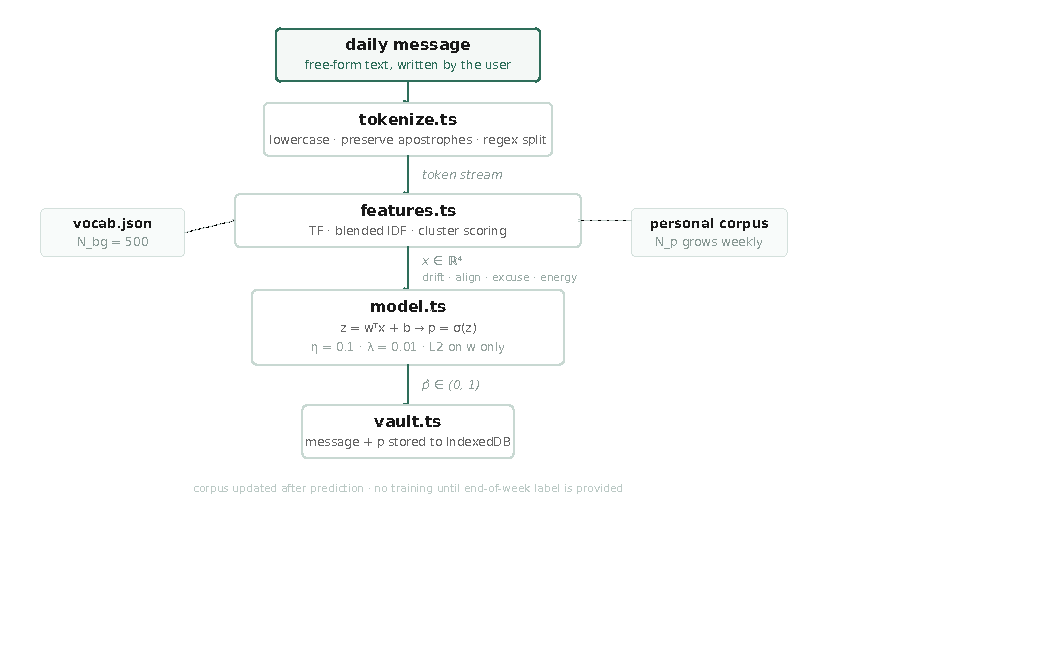
\includegraphics[width=0.72\textwidth, trim=0 9 0 0, clip]{fig_pipeline}
\caption{Data flow for a single daily message submission.}
\label{fig:pipeline}
\end{figure}

% ─────────────────────────────────────────────────────────────────────────────
\chapter{Implementation}
% ─────────────────────────────────────────────────────────────────────────────

\section{Module Overview}

Table~\ref{tab:modules} lists every implementation file with its module
and responsibility.

\begin{table}[H]
\centering
\caption{Implementation modules}
\label{tab:modules}
\begin{tabularx}{\textwidth}{@{} p{2.6cm} p{2.0cm} X @{}}
\toprule
\textbf{File} & \textbf{Module} & \textbf{Responsibility} \\
\midrule
\texttt{types.ts}      & frisbee & Type definitions shared across the ML pipeline. \\
\texttt{tokenize.ts}   & frisbee & Apostrophe-preserving tokeniser. \\
\texttt{features.ts}   & frisbee & Blended IDF feature extractor. \\
\texttt{model.ts}      & frisbee & Logistic regression: predict, loss, gradient step. \\
\texttt{scientist.ts}  & frisbee & Word-delta hypothesis surfacing. \\
\texttt{vault.ts}      & frisbee & IndexedDB persistence layer. \\
\texttt{engine.ts}     & frisbee & Orchestration: message submission and weekly training. \\
\texttt{vocab.json}    & frisbee & Hand-curated cluster words and background corpus. \\
\midrule
\texttt{bus.ts}        & buddy  & Typed pub/sub event bus. \\
\texttt{brain.ts}      & buddy  & Mascot state machine (Zustand). \\
\texttt{fx.ts}         & buddy  & Web Audio API and haptics layer. \\
\texttt{voice.ts}      & buddy  & Response lexicon and selection. \\
\bottomrule
\end{tabularx}
\end{table}

\section{The ML Pipeline}

\subsection{engine.ts}

The engine is the only entry point from the UI into the ML pipeline. It
exposes two asynchronous functions. \texttt{submitMessage(text)} tokenises
the input, extracts the feature vector, generates the prediction, stores
the message to the vault, and updates the personal corpus. The corpus
update uses only the unique tokens from the submitted message: each unique
word increments $df_p$ by one. Crucially, the corpus update occurs after
prediction, so the current message does not influence its own IDF weights.

\texttt{trainOnWeek(week)} retrieves all messages for the given week start
timestamp and runs one gradient step per message in chronological order.
The model state is written back to IndexedDB after the final step of the
epoch.

The function \texttt{weekStartOf(ts)} computes Monday 00:00 local time for
any given Unix timestamp. This value serves as the primary key for week
records, ensuring messages from the same calendar week are consistently
grouped regardless of when they were submitted.

\subsection{model.ts}

The gradient step is the core computation of the system. Algorithm~\ref{alg:step}
presents the procedure.

\begin{algorithm}[H]
\caption{Single gradient step}
\label{alg:step}
\begin{algorithmic}[1]
\Require model $(\mathbf{w}, b)$, feature vector $\mathbf{x}$,
         truth $y \in \{0,1\}$, $\eta = 0.1$, $\lambda = 0.01$
\State $z \leftarrow \mathrm{clip}(\mathbf{w}^\top\mathbf{x} + b,\;
       -500,\; 500)$
\State $\hat{p} \leftarrow 1/(1 + e^{-z})$
\State $\mathrm{err} \leftarrow \hat{p} - y$
\For{$i = 1$ to $4$}
  \State $w_i \leftarrow w_i
         - \eta\,\mathrm{err}\,x_i
         - \eta\,\lambda\,w_i$
         \Comment{L2 on weights only}
\EndFor
\State $b \leftarrow b - \eta\,\mathrm{err}$
       \Comment{no regularisation on bias}
\State \Return updated $(\mathbf{w}, b)$
\end{algorithmic}
\end{algorithm}

The step function does not mutate its input. It returns a new model state
object and increments the update counter. This makes the training history
traceable from the stored state.

A Python reference implementation (\texttt{collect.py}) applies the same
formulae, and a parity test enforces byte-identical feature vectors for
identical inputs across both languages. This confirms that the mathematical
specification in Chapter~3 is implemented without approximation.

\section{The Event Bus}

\texttt{bus.ts} is a zero-dependency publish/subscribe module. It maintains
a \texttt{Map} from event type to a \texttt{Set} of handler functions. The
full event type union is a TypeScript discriminated union, giving each
subscriber complete type narrowing when it inspects the event type before
accessing payload fields. This is why no subscriber in the codebase requires
a runtime cast.

The disposer returned by \texttt{on()} re-resolves the set from the map at
call time rather than closing over the local reference at registration time:

\smallskip
\centerline{\texttt{return () => subs.get(type)?.delete(fn);}}
\smallskip

This ensures that if the underlying \texttt{Set} were ever replaced in a
refactor, the disposer would still work correctly rather than silently
becoming a no-op and leaking subscriptions.

\section{The Buddy Layer}

\subsection{brain.ts}

The mascot brain is a Zustand state machine with eight moods. Moods decay
back to \textit{neutral} after a configurable time-to-live via a
module-level timer. The function \texttt{dominantCluster} maps the feature
vector $\mathbf{x}$ to a mascot reaction by selecting the cluster with the
highest score. This is the only point at which ML output influences UX
behaviour; the mascot never reads model weights or probabilities directly.

\subsection{fx.ts}

The sound layer generates audio via the Web Audio API using no audio files.
Each event produces one or more oscillator nodes with amplitude envelopes
tuned for the event type. Haptic feedback is provided via
\texttt{navigator.vibrate} where available. The audio context is created
only after the first user gesture, respecting browser autoplay restrictions.

\subsection{voice.ts}

The response lexicon is compiled with the TypeScript \texttt{as const}
assertion, which narrows every string array to its exact literal types.
Without this, the \texttt{pick()} function returns \texttt{string} and the
compiler cannot catch missing or misspelled keys at build time. The
\texttt{pick()} function accepts an optional integer seed for deterministic
selection, useful for preventing response flicker on re-render.

\section{Application Routes}

The application has five routes, shown in Figure~\ref{fig:routes}.

\begin{figure}[H]
\centering
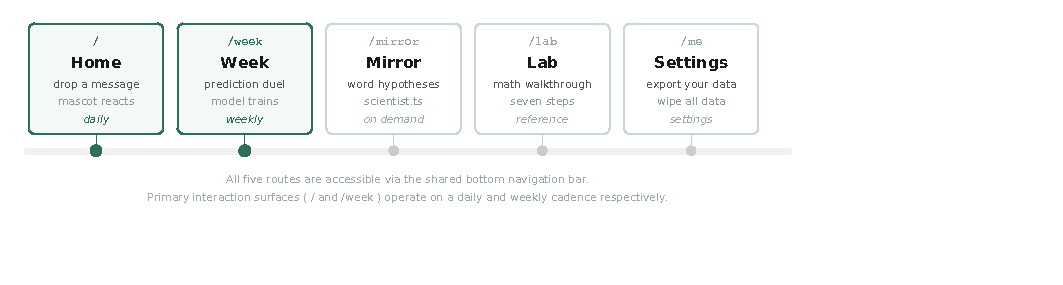
\includegraphics[width=\textwidth, trim=0 7 0 0, clip]{fig_routes}
\caption{Application routes and shared bottom navigation bar.}
\label{fig:routes}
\end{figure}

\section{The Weekly Cycle}

Figure~\ref{fig:cycle} shows the complete prediction and training loop
that the user moves through each week.

\begin{figure}[H]
\centering
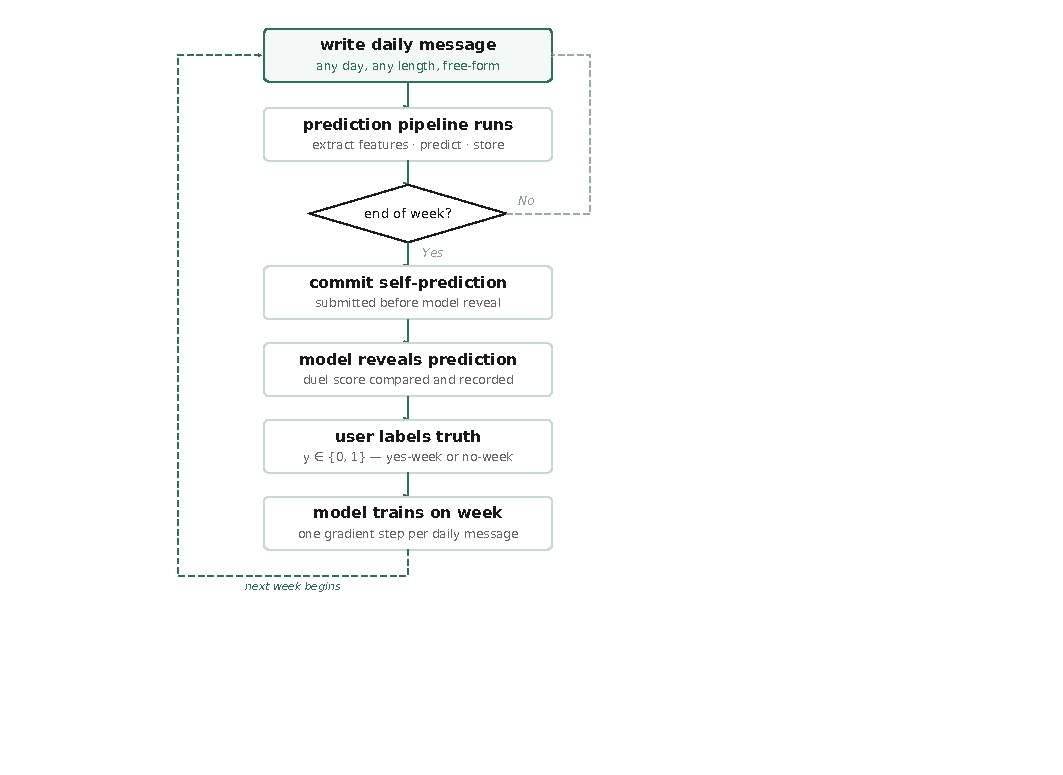
\includegraphics[width=0.62\textwidth, trim=0 11 0 0, clip]{fig_cycle}
\caption{Weekly prediction and training cycle.}
\label{fig:cycle}
\end{figure}

% ─────────────────────────────────────────────────────────────────────────────

\clearpage
% ─────────────────────────────────────────────────────────────────────────────
\chapter{Results and Discussion}
% ─────────────────────────────────────────────────────────────────────────────

\section{MVP Status}

The current implementation is a fully functional minimum viable product,
deployed at \texttt{myfrisbee.lovable.app}. All modules described in
Chapters 3 and 4 are operational. The system correctly tokenises daily
messages, extracts feature vectors, generates predictions, stores data to
IndexedDB, and updates model weights after each weekly training event.
The prediction duel is live: the user submits a self-prediction, the model
reveals its own, and the score is tracked across weeks.

No multi-week longitudinal data was collected during the development
period. The results in this chapter are therefore analytical. They describe
the expected behaviour of the system based on the mathematics of the model
and the structure of the implementation.

\section{Expected Performance}

\subsection{Cold Start}

In the first few weeks, $N_p$ is small and the blended IDF is dominated
by the background corpus. The weights $\mathbf{w}$ are initialised to
zero, so $\hat{p} = \sigma(0) = 0.5$ on the first message. Both the model
and the user are making near-chance predictions at this stage, so the duel
score will tend toward \textit{both wrong} or \textit{both right}
roughly equally.

\subsection{Convergence}

As $N_p$ grows, the personal IDF progressively dominates the blend and
the feature vectors become more discriminative. The model will begin to
assign consistent weight to words that reliably co-occur with yes-weeks
or no-weeks for this specific user. The magnitude of weight updates,
$\|\Delta\mathbf{w}\|$, will rise initially and then stabilise as the
weights converge. Table~\ref{tab:phases} summarises the expected
behaviour by phase.

\begin{table}[H]
\centering
\caption{Expected model behaviour by phase}
\label{tab:phases}
{\small
\begin{tabularx}{\textwidth}{@{} p{2.2cm} p{2.0cm} X @{}}
\toprule
\textbf{Phase} & \textbf{Weeks} & \textbf{Expected behaviour} \\
\midrule
Cold start   & 1--3   & Background IDF dominates. $\hat{p} \approx 0.5$.
                        Both model and user at near chance. \\[4pt]
Learning     & 4--10  & Personal IDF asserts. Weights shift from zero.
                        Predictions grow more confident. \\[4pt]
Convergence  & 10+    & Weights stabilise. Model MAE expected to fall
                        below user self-prediction MAE. \\
\bottomrule
\end{tabularx}}
\end{table}

\subsection{Primary Metric: MAE}

The primary evaluation metric is mean absolute error between the binary
prediction and the ground truth over a held-out test period. For the model
and the user respectively:
\begin{equation}
  \mathrm{MAE}_{\mathrm{model}}
  = \frac{1}{T}\sum_{t=1}^{T}|\hat{p}_t^{\mathrm{rounded}} - y_t|
  \qquad
  \mathrm{MAE}_{\mathrm{user}}
  = \frac{1}{T}\sum_{t=1}^{T}|s_t - y_t|
\end{equation}

where $s_t$ is the user's self-prediction and $y_t$ is the ground truth
for week $t$. A four-week held-out period ($T=4$) is planned. This is a
proof-of-concept scale: the sample is too small for significance testing,
but it is sufficient to observe the direction of the comparison.

\section{Limitations}

\begin{enumerate}
  \item \textbf{No longitudinal data.} The system has not been evaluated
    over a complete multi-week period with real user data. All expected
    performance figures are analytical.

  \item \textbf{Fixed vocabulary.} The cluster word lists are hand-curated.
    A user whose language falls outside these lists will produce weak
    feature vectors regardless of model quality. The user can add words
    via \texttt{/me}, but the base coverage is fixed at build time.

  \item \textbf{Self-report bias.} The label $y$ is user-provided at
    week end. Mood at labelling time can distort the signal: a difficult
    Sunday may retroactively make a neutral week feel like a no-week.

  \item \textbf{Binary outcome.} Modelling alignment as a binary variable
    discards gradations. A week that was \textit{almost} a yes-week and
    a clearly failed week receive identical labels.

  \item \textbf{No confidence display.} The application shows the model's
    binary prediction but not $\hat{p}$. Per \citet{hengstler2016},
    showing calibrated confidence supports adaptive trust calibration.
    This is currently absent.
\end{enumerate}

\clearpage
% ─────────────────────────────────────────────────────────────────────────────
\chapter{Conclusion}
% ─────────────────────────────────────────────────────────────────────────────

\section{Summary}

FRISBEE demonstrates that a logistic regression model trained exclusively
on one person's daily free-form text can learn their specific behavioural
language patterns over time. The system operationalises a narrow but
well-founded hypothesis: that the gap between a person's self-prediction
and their actual behaviour is consistent enough, and linguistically
detectable enough, to be modelled at the individual level.

The key technical contributions are: a blended inverse document frequency
formula that resolves the cold-start problem from day one; a training
protocol that updates the model once per daily message per week rather
than once per week; L2 regularisation applied to the weight vector only,
preserving the bias as a learnable base rate; and a fully on-device
architecture with no server component and no data transmission.

The minimum viable product is live. The system works as designed.

\section{Future Work}

\begin{enumerate}
  \item \textbf{Longitudinal evaluation.} Run the system over twelve or
    more weeks with real users and report MAE comparisons between model
    and self-prediction. This is the study the hypothesis requires.

  \item \textbf{Dynamic vocabulary.} Let the model surface user-specific
    signal words from message history and propose them for addition to
    the relevant cluster. This extends the fixed vocabulary toward
    personalised feature discovery.

  \item \textbf{Temporal decay.} Weight recent messages more heavily.
    Behavioural patterns shift over months; old labels should carry less
    influence on current predictions.

  \item \textbf{Confidence display.} Surface $\hat{p}$ alongside the
    binary prediction, framed in plain language. Per \citet{hengstler2016},
    this is the correct path to adaptive trust calibration.

  \item \textbf{Multi-user study.} Run FRISBEE across a cohort. Individual
    models stay private. Aggregate MAE comparisons would constitute
    statistically meaningful evidence for or against the central hypothesis.

  \item \textbf{Cognitive load signal.} Use message length and vocabulary
    diversity as a proxy for cognitive load, per \citet{sweller1988}.
    A secondary feature may improve prediction accuracy on weeks where
    emotional state, not language pattern, drives behaviour.
\end{enumerate}

% ─────────────────────────────────────────────────────────────────────────────

\bibliographystyle{plainnat}
\bibliography{refs}

\end{document}
